% 1977 年江苏常州市初试卷第 10 题：圆 O 与两条割线——过圆心的割线 P-D-O-C，
% 圆外一点 P 的割线 P-B-A（按源卷第 2 页布局）
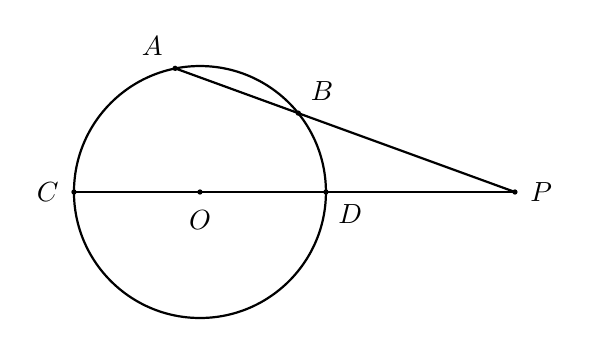
\begin{tikzpicture}[scale=0.8]
  \coordinate (O) at (0,0);
  \coordinate (P) at (5,0);
  \coordinate (C) at (-2,0);
  \coordinate (D) at (2,0);
  \coordinate (B) at (1.561,1.252);
  \coordinate (A) at (-0.394,1.963);
  \draw[thick] (0,0) circle (2);
  \draw[thick] (C)--(P);
  \draw[thick] (P)--(A);
  \fill (O) circle (1.2pt) node[below=3pt] {$O$};
  \fill (P) circle (1.2pt) node[right=2pt] {$P$};
  \fill (C) circle (1.2pt) node[left=2pt] {$C$};
  \fill (D) circle (1.2pt) node[below right=1pt] {$D$};
  \fill (B) circle (1.2pt) node[above right=1pt] {$B$};
  \fill (A) circle (1.2pt) node[above left=1pt] {$A$};
\end{tikzpicture}
